\documentclass[aspectratio=169,11pt,xcolor=table]{beamer}

\usetheme{default}
\usecolortheme{default}
\setbeamertemplate{navigation symbols}{}
\setbeamertemplate{footline}[frame number]
\setbeamercolor{title}{fg=black}
\setbeamercolor{frametitle}{fg=black,bg=white}
\setbeamercolor{block title}{fg=black,bg=black!8}
\setbeamercolor{block body}{fg=black,bg=black!3}
\setbeamerfont{frametitle}{series=\bfseries,size=\Large}
\setbeamerfont{title}{series=\bfseries,size=\LARGE}

\usepackage[utf8]{inputenc}
\usepackage[T1]{fontenc}
\usepackage{amsmath,amssymb,bm}
\usepackage{booktabs}
\usepackage{array}
\usepackage{tikz}
\usetikzlibrary{shapes.geometric}
\usepackage{pgfplots}
\usepackage{graphicx}
\usepackage{hyperref}
\pgfplotsset{compat=1.18}
\usetikzlibrary{arrows.meta,positioning,calc,fit,matrix}

% -----------------------------------------------------------------------------
% Raster palette
% -----------------------------------------------------------------------------
\definecolor{lowblue}{RGB}{225,240,255}
\definecolor{midblue}{RGB}{120,180,230}
\definecolor{highblue}{RGB}{15,90,160}
\definecolor{lowgreen}{RGB}{230,245,230}
\definecolor{midgreen}{RGB}{120,190,120}
\definecolor{highgreen}{RGB}{20,120,40}
\definecolor{loworange}{RGB}{255,240,220}
\definecolor{midorange}{RGB}{245,170,80}
\definecolor{highorange}{RGB}{190,80,20}
\definecolor{lowred}{RGB}{255,230,230}
\definecolor{midred}{RGB}{240,120,120}
\definecolor{highred}{RGB}{170,20,40}
\definecolor{purpleA}{RGB}{235,225,245}
\definecolor{purpleB}{RGB}{165,120,200}
\definecolor{purpleC}{RGB}{90,40,140}
\definecolor{marginA}{RGB}{245,245,210}
\definecolor{marginB}{RGB}{220,205,95}
\definecolor{marginC}{RGB}{145,120,20}

\newcommand{\cellbox}[2]{\fill[#1] #2 rectangle ++(0.8,0.8);}
\newcommand{\gridframe}{\draw[black!40,step=0.8] (0,0) grid (4,4);}
\newcommand{\rastlabel}[1]{\node[font=\scriptsize,align=center] at (2,-0.35) {#1};}
\newcommand{\smalltag}[1]{\node[font=\tiny,align=center,text=black!65] at (2,4.35) {#1};}

\newcommand{\bigquote}[1]{%
	\begin{center}
		\begin{minipage}{0.88\linewidth}
			\centering\Large\itshape #1
		\end{minipage}
\end{center}}

\title{Two-Timescale Resilience}
\subtitle{Mapping the Contraction of Biological Viability Bounds}
\author{Stijn H. Peeters}
\date{\today}

\begin{document}
	
	\begin{frame}
		\titlepage
		\vspace{-0.8em}
	\end{frame}
	
	\begin{frame}{The Pressure Manifold}
		\begin{center}
			How do we construct a pressure manifold: a many-input device that funnels qualitatively different burdens \textit{into} an account of health?
			
			\vspace{1.2em}
			
			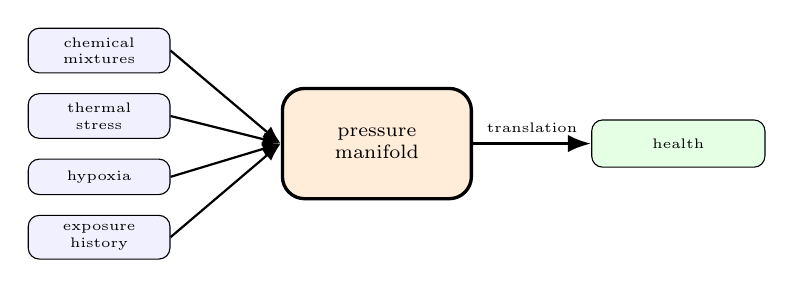
\begin{tikzpicture}[
				>=Latex,
				node distance=0.7cm,
				input/.style={
					draw,
					rounded corners,
					align=center,
					font=\tiny,
					minimum width=1.8cm,
					minimum height=0.45cm,
					fill=blue!6
				},
				manifold/.style={
					draw,
					rounded corners=8pt,
					align=center,
					font=\scriptsize,
					minimum width=2.4cm,
					minimum height=1.4cm,
					fill=orange!15,
					very thick
				},
				output/.style={
					draw,
					rounded corners,
					align=center,
					font=\tiny,
					minimum width=2.2cm,
					minimum height=0.6cm,
					fill=green!10
				}
				]
				
				% Inputs
				\node[input] (chem) {chemical\\mixtures};
				\node[input,below=0.25cm of chem] (temp) {thermal\\stress};
				\node[input,below=0.25cm of temp] (hypoxia) {hypoxia};
				\node[input,below=0.25cm of hypoxia] (memory) {exposure\\history};
				
				% Manifold
				\node[manifold,right=1.4cm of temp,yshift=-0.35cm] (man)
				{pressure\\manifold};
				
				% Output
				\node[output,right=1.5cm of man] (health)
				{health};
				
				% Arrows into manifold
				\draw[->,thick] (chem.east) -- (man.west);
				\draw[->,thick] (temp.east) -- (man.west);
				\draw[->,thick] (hypoxia.east) -- (man.west);
				\draw[->,thick] (memory.east) -- (man.west);
				
				% Arrow out
				\draw[->,very thick] (man.east) -- node[above,font=\tiny] {translation} (health.west);
				
			\end{tikzpicture}
			
			\vspace{1em}
			
			\small without resorting to \textit{regulatory} limits as the \textit{stand-in} for ``health''.
		\end{center}
	\end{frame}
	
	\begin{frame}{The Regulatory Trap}
		\begin{center}
			\Large What is Health? 
		\end{center}
		
		\vspace{1em}
		
		In standard ecotoxicology, health is posited as a negative: \textbf{the absence of a threshold exceedance.}
		
		\vspace{1em}
		
		\begin{quote}
			\textit{"The organism is treated as a rigid fortress defending a baseline. This is not health; it is the description of a pathology."}
		\end{quote}
	\end{frame}
	
	\begin{frame}{Canguilhem: Health as Normative Capacity}
		\begin{columns}[T,onlytextwidth]
			\begin{column}{0.34\textwidth}
				
				\IfFileExists{Canguilhem.jpg}{%
					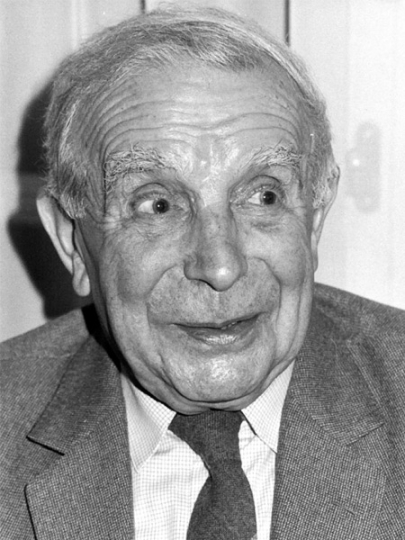
\includegraphics[width=0.82\linewidth]{Canguilhem.jpg}
				}{%
					
\begin{tikzpicture}
						\node[draw,rounded corners,minimum width=3.6cm,minimum height=4.4cm,fill=black!4,align=center] {Canguilhem\\image here};
					\end{tikzpicture}
				}
			\end{column}
			\begin{column}{0.63\textwidth}
				
				\centering
				\Large \textit{Health is normativity.}
				
				\vspace{1em}
				
				\normalsize True biological health is the positive, creative capacity to tolerate environmental shocks, absorb an engulfing medium, and establish a \textbf{new biological norm}.
				\vspace{1em}
				
				\Large "\textit{A state $\ldots$ which the living being's every anxious effort will tend to preserve from every eventual disturbance.}"
				
			\end{column}
		\end{columns}
	\end{frame}
	
	\begin{frame}{Energy as the Currency of Capacity}
		
		\vspace{0.7em}
		
		\begin{block}{The Thermodynamic Assumption}
			A norm transformation is accessible only if the biological system has enough \textbf{energetic luxury} to pay for it.
		\end{block}
		
		\begin{block}{The Mechanistic Translation}
			How do we go from chemical concentrations to a quantifiable loss of norm-generating capacity?
		\end{block}
		
	\end{frame}
	
	\begin{frame}{Dynamic Energy Budget (DEB) Engine}
		\begin{center}
			
			\vspace{0.4em}
			
			\normalsize We map the phenomenological pressure of the environment into DEB thermodynamic taxes to estimate remaining \textbf{Adaptive Margin}.
			
			\vspace{1.2em}
			
			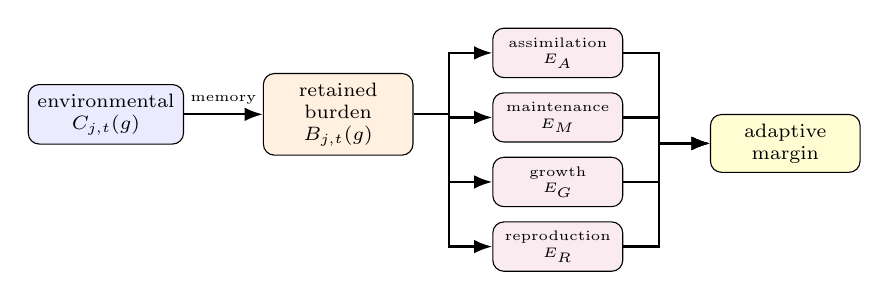
\begin{tikzpicture}[
				>=Latex,
				node distance=0.7cm,
				box/.style={
					draw,
					rounded corners,
					align=center,
					minimum width=1.9cm,
					minimum height=0.58cm,
					font=\scriptsize
				},
				axis/.style={
					draw,
					rounded corners,
					align=center,
					minimum width=1.65cm,
					minimum height=0.48cm,
					font=\tiny,
					fill=purple!8
				}
				]
				
				\node[box,fill=blue!8] (C)
				{environmental\\$C_{j,t}(g)$};
				
				\node[box,fill=orange!12,right=1.0cm of C] (B)
				{retained\\burden\\$B_{j,t}(g)$};
				
				\node[axis,right=1.0cm of B,yshift=0.78cm] (assim)
				{assimilation\\$E_A$};
				
				\node[axis,below=0.18cm of assim] (maint)
				{maintenance\\$E_M$};
				
				\node[axis,below=0.18cm of maint] (growth)
				{growth\\$E_G$};
				
				\node[axis,below=0.18cm of growth] (repr)
				{reproduction\\$E_R$};
				
				\node[box,fill=yellow!18,right=1.1cm of maint,yshift=-0.33cm] (margin)
				{adaptive\\margin};
				
				\draw[->,thick] (C) -- node[above,font=\tiny] {memory} (B);
				
				\draw[->,thick] (B.east) -- ++(0.45,0) |- (assim.west);
				\draw[->,thick] (B.east) -- ++(0.45,0) |- (maint.west);
				\draw[->,thick] (B.east) -- ++(0.45,0) |- (growth.west);
				\draw[->,thick] (B.east) -- ++(0.45,0) |- (repr.west);
				
				\draw[->,thick] (assim.east) -- ++(0.45,0) |- (margin.west);
				\draw[->,thick] (maint.east) -- ++(0.45,0) |- (margin.west);
				\draw[->,thick] (growth.east) -- ++(0.45,0) |- (margin.west);
				\draw[->,thick] (repr.east) -- ++(0.45,0) |- (margin.west);
				
			\end{tikzpicture}
			
			\vspace{0.6em}
			
			\small Adaptive Margin is the remaining energetic distance between what the organism can mobilize, and what it \textbf{must} spend to stay alive.
			
		\end{center}
	\end{frame}
	
	
	\begin{frame}{From Adaptive Margin to Amplification}
		\begin{center}
			
			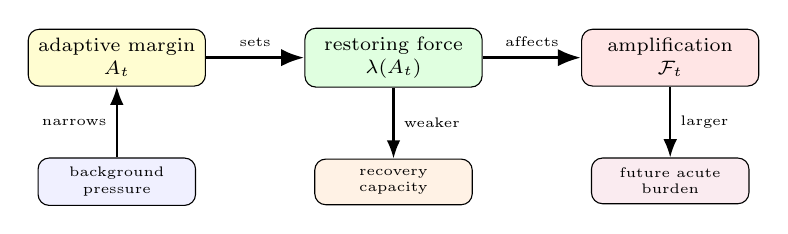
\begin{tikzpicture}[
				>=Latex,
				node distance=1.1cm,
				box/.style={
					draw,
					rounded corners,
					align=center,
					minimum width=2.25cm,
					minimum height=0.72cm,
					font=\scriptsize
				},
				smallbox/.style={
					draw,
					rounded corners,
					align=center,
					minimum width=2.0cm,
					minimum height=0.58cm,
					font=\tiny
				}
				]
				
				\node[box,fill=yellow!18] (A)
				{adaptive margin\\$A_t$};
				
				\node[box,fill=green!12,right=1.25cm of A] (lambda)
				{restoring force\\$\lambda(A_t)$};
				
				\node[box,fill=red!10,right=1.25cm of lambda] (F)
				{amplification\\$\mathcal{F}_t$};
				
				\draw[->,very thick] (A) -- node[above,font=\tiny] {sets} (lambda);
				\draw[->,very thick] (lambda) -- node[above,font=\tiny] {affects} (F);
				
				\node[smallbox,fill=blue!6,below=0.9cm of A] (pressure)
				{background\\pressure};
				
				\node[smallbox,fill=orange!10,below=0.9cm of lambda] (recovery)
				{recovery\\capacity};
				
				\node[smallbox,fill=purple!8,below=0.9cm of F] (burden)
				{future acute\\burden};
				
				\draw[->,thick] (pressure.north) -- node[left,font=\tiny] {narrows} (A.south);
				\draw[->,thick] (lambda.south) -- node[right,font=\tiny] {weaker} (recovery.north);
				\draw[->,thick] (F.south) -- node[right,font=\tiny] {larger} (burden.north);
				
			\end{tikzpicture}
			
			\vspace{1.0em}
			
			\[
			\lambda(A_t)
			=
			\lambda_{\min}
			+
			(\lambda_{\max}-\lambda_{\min})
			\frac{\max(A_t,0)}{K_A+\max(A_t,0)}
			\]
			
			\vspace{-0.4em}
			
			\[
			\mathcal{F}_t
			=
			\frac{\lambda(A_0)}{\lambda(A_t)}
			\]
			
			\vspace{0.2em}
			
			\small
			Lower adaptive margin means weaker recovery; weaker recovery means a larger burden from the same acute event.
			
		\end{center}
	\end{frame}
	
	
	\begin{frame}{The Epistemic Architecture}
		
		\begin{center}
			\resizebox{0.91\linewidth}{!}{%
				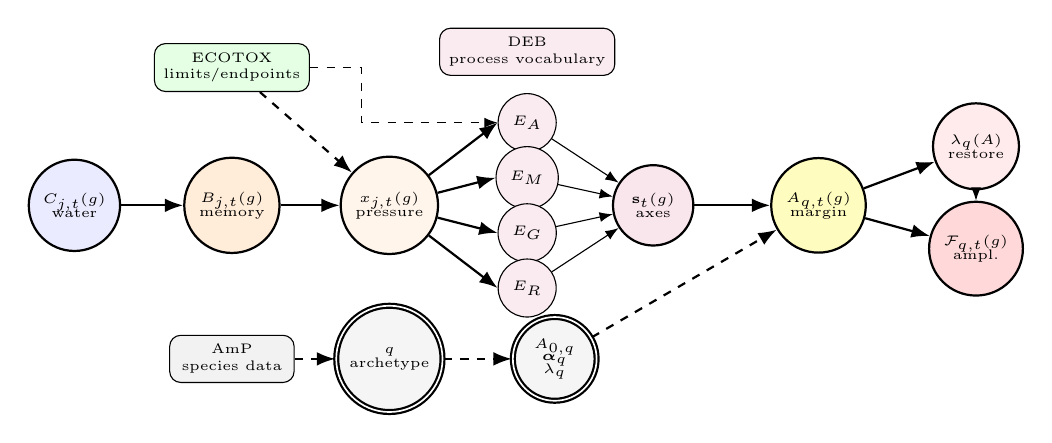
\begin{tikzpicture}[
					>=Latex,
					state/.style={
						circle,
						draw,
						thick,
						align=center,
						minimum size=1.02cm,
						font=\tiny
					},
					evidence/.style={
						rectangle,
						draw,
						rounded corners,
						align=center,
						minimum width=1.58cm,
						minimum height=0.56cm,
						font=\tiny
					},
					species/.style={
						circle,
						double,
						draw,
						thick,
						align=center,
						minimum size=1.02cm,
						font=\tiny
					},
					axisnode/.style={
						circle,
						draw,
						align=center,
						minimum size=0.72cm,
						font=\tiny
					}
					]
					
					% States
					\node[state,fill=blue!8] (C) at (0,0) {$C_{j,t}(g)$\\[-0.15em]water};
					\node[state,fill=orange!15] (B) at (2.0,0) {$B_{j,t}(g)$\\[-0.15em]memory};
					\node[state,fill=orange!8] (U) at (4.0,0) {$x_{j,t}(g)$\\[-0.15em]pressure};
					
					\node[axisnode,fill=purple!8] (EA) at (5.75,1.05) {$E_A$};
					\node[axisnode,fill=purple!8] (EM) at (5.75,0.35) {$E_M$};
					\node[axisnode,fill=purple!8] (EG) at (5.75,-0.35) {$E_G$};
					\node[axisnode,fill=purple!8] (ER) at (5.75,-1.05) {$E_R$};
					
					\node[state,fill=purple!10] (Evec) at (7.35,0) {$\mathbf{s}_t(g)$\\[-0.15em]axes};
					\node[state,fill=yellow!25] (A) at (9.45,0) {$A_{q,t}(g)$\\[-0.15em]margin};
					\node[state,fill=red!15] (F) at (11.45,-0.55) {$\mathcal{F}_{q,t}(g)$\\[-0.15em]ampl.};
					\node[state,fill=red!8] (LAMBDA) at (11.45,0.75) {$\lambda_q(A)$\\[-0.15em]restore};
					
					% Evidence
					\node[evidence,fill=green!10] (ECO) at (2.0,1.75) {ECOTOX\\limits/endpoints};
					\node[evidence,fill=purple!8] (DEB) at (5.75,1.95) {DEB\\process vocabulary};
					\node[evidence,fill=black!5] (AMP) at (2.0,-1.95) {AmP\\species data};
					\node[species,fill=black!4] (Q) at (4.0,-1.95) {$q$\\[-0.15em]archetype};
					\node[species,fill=black!4] (PARAM) at (6.1,-1.95) {$A_{0,q}$\\[-0.2em]$\boldsymbol{\alpha}_q$\\[-0.2em]$\lambda_q$};
					
					% Dynamics
					\draw[->,thick] (C) -- (B);
					\draw[->,thick] (B) -- (U);
					\draw[->,thick] (U) -- (EA.west);
					\draw[->,thick] (U) -- (EM.west);
					\draw[->,thick] (U) -- (EG.west);
					\draw[->,thick] (U) -- (ER.west);
					\draw[->,thin] (EA) -- (Evec);
					\draw[->,thin] (EM) -- (Evec);
					\draw[->,thin] (EG) -- (Evec);
					\draw[->,thin] (ER) -- (Evec);
					\draw[->,thick] (Evec) -- (A);
					\draw[->,thick] (A) -- (LAMBDA);
					\draw[->,thick] (A) -- (F);
					\draw[->,thin,dashed] (LAMBDA) -- (F);
					
					% Evidence Links
					\draw[->,thick,dashed] (ECO) -- (U);
					\draw[->,thin,dashed] (ECO.east) -- ++(0.65,0) |- (EA.west);
					\draw[->,thick,dashed] (AMP) -- (Q);
					\draw[->,thick,dashed] (Q) -- (PARAM);
					\draw[->,thick,dashed] (PARAM) -- (A);
					
			\end{tikzpicture}}
		\end{center}
		\vspace{0.5em}
		\begin{itemize}
			\scriptsize
			\item \textbf{The Commitment:} We collapse DEB state-space matrices into a single macroscopic scalar ($A_t$). 
			\item \textbf{The Trade-off:} We trade microscopic precision for spatial tractability. We model the \textit{envelope of viability}, not exact life history.
		\end{itemize}
	\end{frame}
	
	\begin{frame}{The Theoretical Envelope in Space}
		\begin{center}
			\textit{Spatial distribution of environmental pressure and resulting capacity.}
		\end{center}
		\vspace{0.5em}
		\begin{center}
			\includegraphics[width=0.8\linewidth]{full_example1.png}
		\end{center}
	\end{frame}
	
	\begin{frame}{Embodied Memory and Biological Scar Tissue}
		\begin{center}
			\textit{Even when external concentration clears, retained internal burden keeps the Adaptive Margin compressed, leaving recovery capacity structurally compromised.}
		\end{center}
		\vspace{0.5em}
		\begin{center}
			\includegraphics[width=0.9\linewidth]{full_example3.png}
		\end{center}
	\end{frame}
	
	\begin{frame}{Closing}
		\bigquote{By fusing DEB theory with AmP data and ECOTOX pressure, we shift the fundamental question.}
		\vspace{0.4em}
		\begin{center}
			\Large We stop asking: \textit{"Is the water toxic?"} \\
			\vspace{0.8em}
			\Large\bfseries And start asking: \textit{"How much adaptive margin remains?"}
		\end{center}
	\end{frame}
	
	\appendix
	\begin{frame}[allowframebreaks]{References}
		\scriptsize
		\begin{thebibliography}{99}
			\bibitem{canguilhem1991normal} Canguilhem, G. (1991). \emph{The Normal and the Pathological}. Zone Books.
			\bibitem{canguilhem2008knowledge} Canguilhem, G. (2008). \emph{Knowledge of Life}. Fordham University Press.
			\bibitem{flusser2012vamp} Flusser, V., \& Bec, L. (2012). \emph{Vampyroteuthis Infernalis: A Treatise, with a Report by the Institut Scientifique de Recherche Paranaturaliste}. University of Minnesota Press.
			\bibitem{kooijman2010deb} Kooijman, S. A. L. M. (2010). \emph{Dynamic Energy Budget Theory for Metabolic Organisation}. Cambridge University Press.
			\bibitem{marques2018amp} Marques, G. M. et al. (2018). The AmP project: comparing species on the basis of Dynamic Energy Budget parameters. \emph{PLOS Computational Biology}, 14(5), e1006100.
			\bibitem{olker2022ecotox} Olker, J. H. et al. (2022). The ECOTOXicology Knowledgebase: a curated database of ecologically relevant toxicity tests. \emph{Scientific Data}, 9, 124.
		\end{thebibliography}
	\end{frame}
	
\end{document}